\documentclass[a4paper]{article}

%% Language and font encodings
\usepackage[english]{babel}
\usepackage[utf8x]{inputenc}
\usepackage[T1]{fontenc}

%% Sets page size and margins
\usepackage[a4paper,top=3cm,bottom=2cm,left=3cm,right=3cm,marginparwidth=1.75cm]{geometry}

%% Useful packages
\usepackage{amsmath}
\usepackage{graphicx}
\usepackage[colorinlistoftodos]{todonotes}
\usepackage[colorlinks=true, allcolors=blue]{hyperref}

%% Comment defs
\newcommand{\nasir}[1]{{\color{blue}#1}}

\title{Mid-project Report}
\author{Team Stylists}

\begin{document}
\maketitle

\section{Task}
Our task is voice conversion/ voice style transfer. We hope to find a latent space where movement encodes audible change in style of audio. In our baseline, we trained a cycleGAN to go between male and female audio data. The results were interesting considering the models trained on raw images. We are currently working on building a cyclic model with a wavenet encoder and/or decoder.

So far we have split our group into two teams each pursuing different approaches. Andrew and Sriram were working with CycleGAN (Sriram also pursuing Wavenet approaches). Meanwhile Nasir and Arshdeep were exploring conditional Wavenets. Moreover, we are also considering the possibility of using a hybrid architecture with contributions from both subgroups.

\section{Data}
We are using the \href{http://homepages.inf.ed.ac.uk/jyamagis/page3/page58/page58.html}{VCTK dataset}. The dataset contains speech from 109 speakers who say approximately 400 sentences from newspapers with wide phonetic and contextual coverage. Audio files are .wav with 48,000 starting sample rate and about a couple of seconds on average in length (about 15 gb of audio). The data is prime for identifying speaker accents and latent space for speaker qualities.

\section{Baseline}
We trained a CycleGAN in Tensorflow on the VCTK dataset. The two collections were male and female audio.
\subsection{Preprocessing and Postprocessing}
A short-time fourier transform was applied on the wav files using librosa and padded to form a 3 channel image of size 256 x 256. The Griffin-Lim algorithm was used for reconstruction of audio from the spectrogram.

\subsection{Training}
The following are results on Google Cloud's K80 GPU instance (12 GB VRAM) after training for a few hours. See Figure \ref{fig:cycleloss}.
\begin{figure}[!htb]
\centering
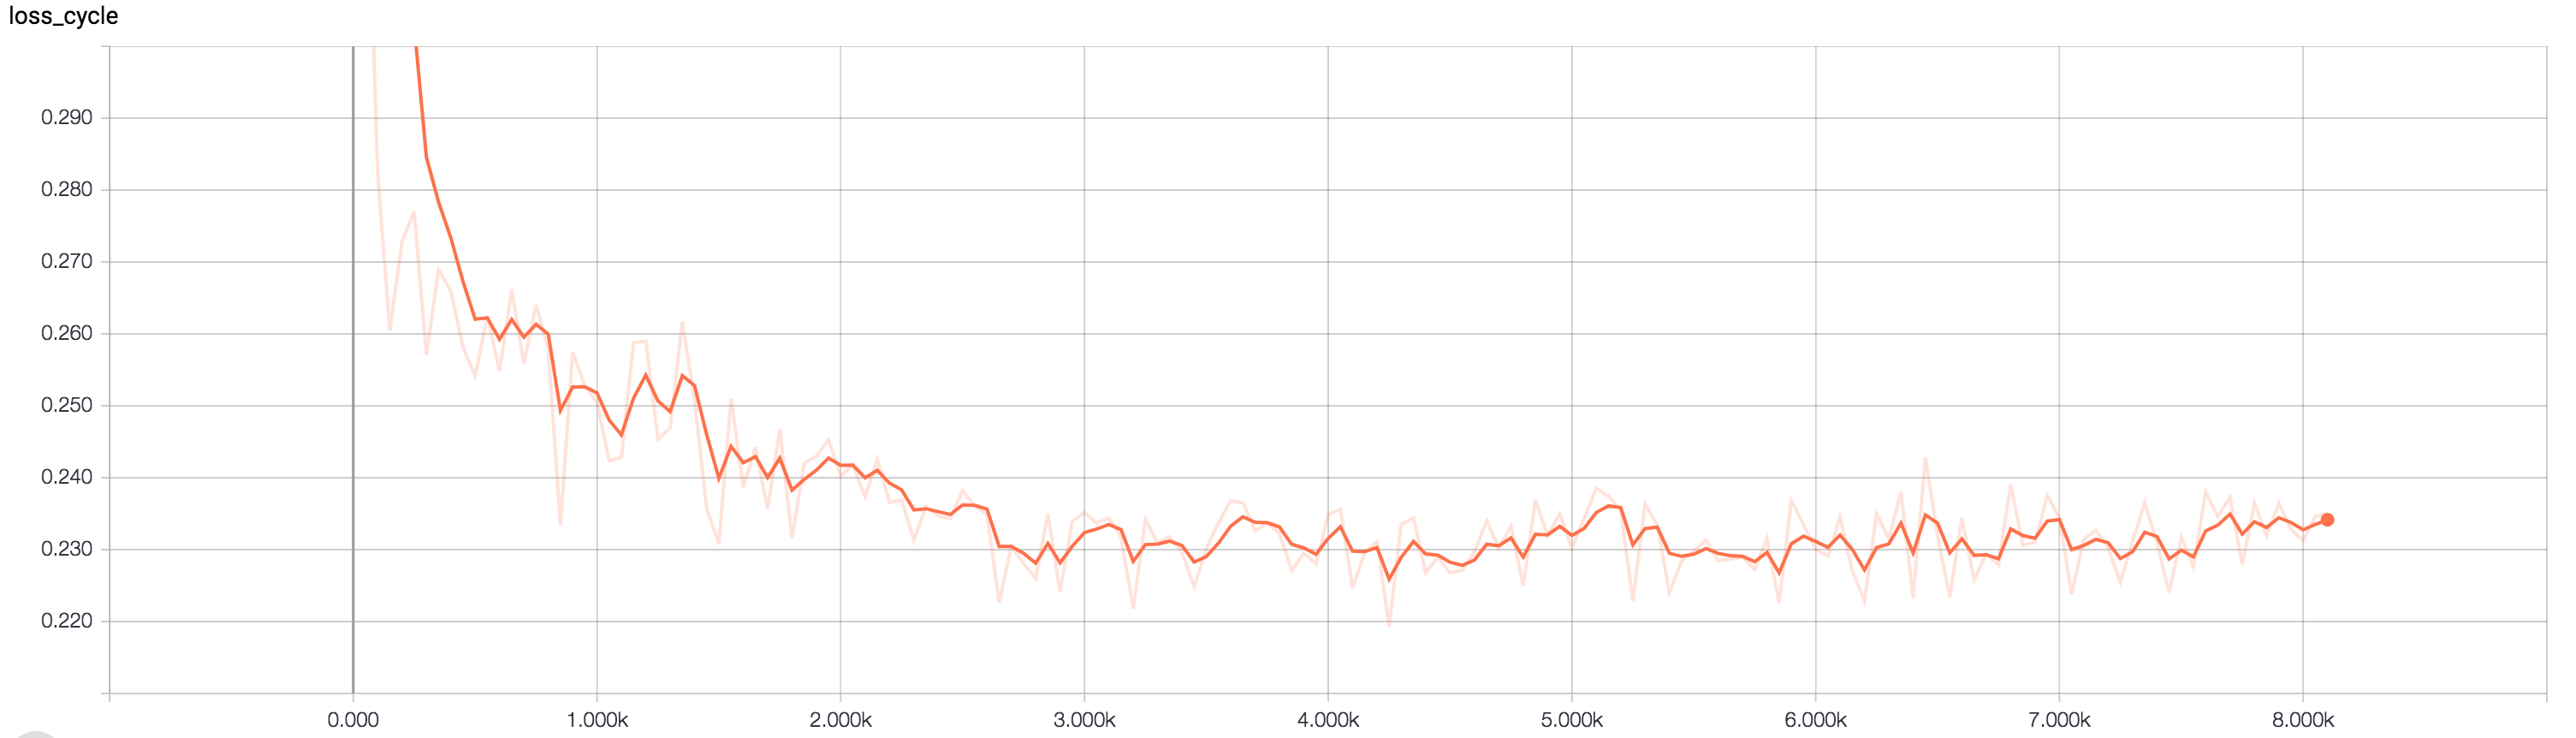
\includegraphics[width=0.8\textwidth]{cyclegan_cycleloss.png}
\caption{\label{fig:cycleloss}Cycle loss for 8k iterations over a couple hours.}
\end{figure}

\begin{figure}[!htb]
\centering
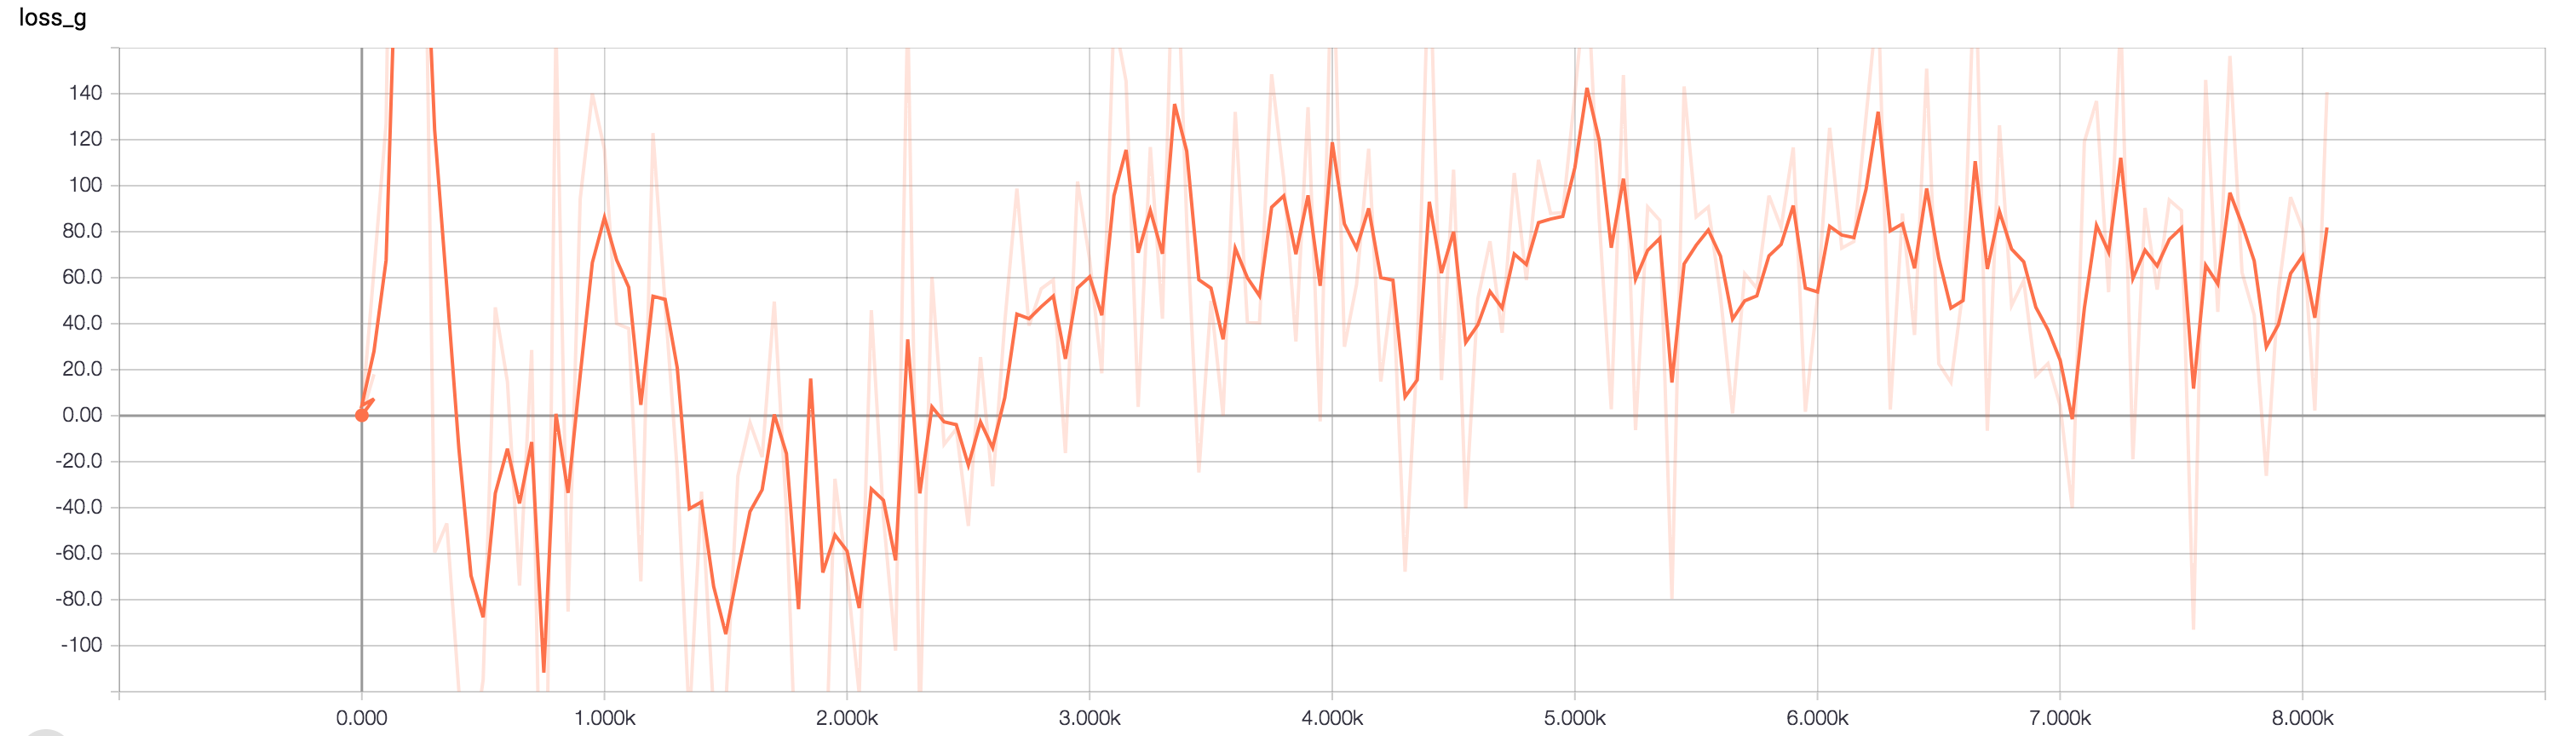
\includegraphics[width=0.8\textwidth]{cyclegan_genloss.png}
\caption{\label{fig:genloss}Generative loss for 8k iterations over a couple hours.}
\end{figure}

The generative loss oscillates (which seems to be the norm for CycleGAN training), whereas the cycle loss steadily decreases. We also trained this same model for 100k iterations using 2 TitanX GPUs. The output result quality for the more trained model was actually more noisy and robotic sounding. 

\subsection{Results and Thoughts}
Generally, we were surprised by the results we got. We weren't expecting much as we were treating the audio spectrogram as images and running a CycleGAN on images of male and female speech from two large collections. However, results after few tens of thousands of iterations comes out grainy but there is a perceivable pitch change from a male and female voice and vice versa.

\begin{figure}[!htb]
\centering
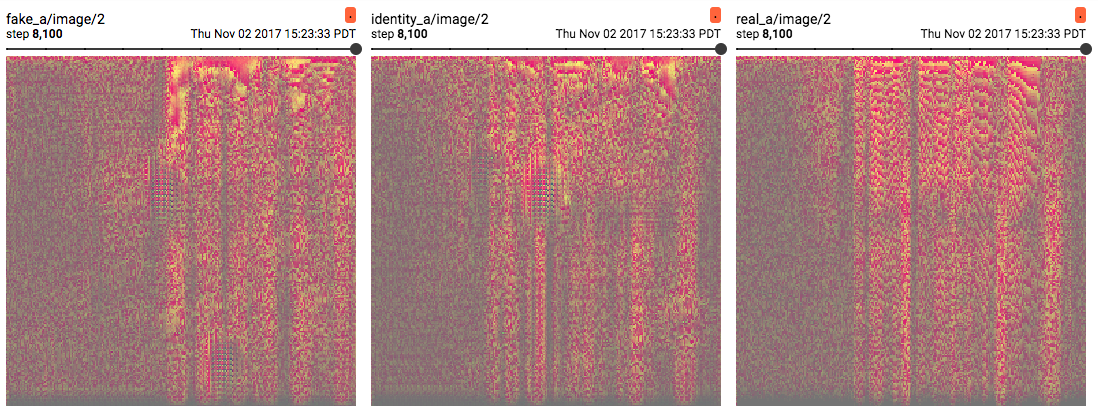
\includegraphics[width=0.8\textwidth]{a_prog_8k.png}
\caption{\label{fig:cycle_comparison}Images of padded audio spectrograms for a male audio sample, fake male audio sample, and reconstructed male sample.}
\end{figure}


\section{Progress}
\subsection{Conditional Wavenet}
Our baseline is clearly hindered by operating on spectrogram data. Wavenet is a powerful model for audio that will work on the raw audio data rather than the spectrogram. Furthermore, we can transfer user voices by conditioning the Wavenet with a user voice style. We have trained a Wavenet model that was globally conditioned on the speaker identifications in the VCTK dataset without getting great results.  

\subsection{Vector Quantised Variational Autoencoder (VQ-VAE)}
A more recent and advanced idea of the conditional Wavenet that we hope to implement is conditioning on both the speaker ID of the style user and the latent space of the content user's voice to "stylize" the content user's voice through Wavenet. The latent space is obtained by VQ-VAE in this case. The paper has been released a few days ago with no code implementation. We plan to implement the paper possibly with a few optimizations. We can use latent space and speaker id to do style transfer.

Recent paper by Deepmind \href{https://arxiv.org/pdf/1711.00937.pdf}{here}.
\end{document}
